% This is a LaTeX thesis template for Monash University.
% to be used with Rmarkdown
% This template was produced by Rob Hyndman
% Version: 6 September 2016

\documentclass{monashthesis}

%%%%%%%%%%%%%%%%%%%%%%%%%%%%%%%%%%%%%%%%%%%%%%%%%%%%%%%%%%%%%%%
% Add any LaTeX packages and other preamble here if required
\usepackage{subcaption}
%%%%%%%%%%%%%%%%%%%%%%%%%%%%%%%%%%%%%%%%%%%%%%%%%%%%%%%%%%%%%%%

\author{Dewi Lestari Amaliah}
\title{Thesis title}
\studentid{31251587}
\def\degreetitle{Master of Business Analytics}
% Add subject and keywords below
\hypersetup{
     %pdfsubject={The Subject},
     %pdfkeywords={Some Keywords},
     pdfauthor={Dewi Lestari Amaliah},
     pdftitle={Thesis title},
     pdfproducer={Bookdown with LaTeX}
}


\bibliography{thesisrefs}

\begin{document}

\pagenumbering{roman}

\titlepage

{\setstretch{1.2}\sf\tighttoc\doublespacing}

\clearpage\pagenumbering{arabic}\setcounter{page}{0}

\hypertarget{abstract}{%
\chapter*{Abstract}\label{abstract}}
\addcontentsline{toc}{chapter}{Abstract}

The abstract should outline the main approach and findings of the thesis and must not be more than 500 words.

\newpage

\hypertarget{acknowledgements}{%
\chapter*{Acknowledgements}\label{acknowledgements}}
\addcontentsline{toc}{chapter}{Acknowledgements}

I would like to thank my pet goldfish for \dots

\hypertarget{ch:intro}{%
\chapter{Introduction}\label{ch:intro}}

\hypertarget{problem-statement}{%
\section{Problem Statement}\label{problem-statement}}

Survey -\textgreater{} MRP -\textgreater{} visualisation

\hypertarget{mrp-overview}{%
\section{MRP Overview}\label{mrp-overview}}

\hypertarget{sec:syslitrev}{%
\chapter{Systematic Literature Review}\label{sec:syslitrev}}

This study is performed using a systematic review method. This method collects empirical evidence explicitly and systematically using pre-specified eligibility criteria to answer a specific research question \autocite{cochrane}. Systematic literature reviews also enable the process of finding the gap in a field of science, such as understanding what has been done and what needs to be done \autocite{LinnenlueckeMartinaK2020Cslr}. Hence, in this case, systematic literature review could assist us to understand the common practice in MRP visualisations so that we can explore how to improve.

According to \textcite{brown_uni}, the key criteria of the systematic literature review are: \emph{``a clearly defined question with inclusion \& exclusion criteria; rigorous \& systematic search of the literature; critical appraisal of included studies; data extraction and management; analysis \& interpretation of results; and report for publication.''} Hence, to conform with these criteria, this study incorporates the Preferred Reporting Items for Systematic Reviews and Meta-Analysis (PRISMA)'s checklist and flow diagram. The following subsections discuss the steps conducted following these criteria.

\hypertarget{literature-identification}{%
\section{Literature Identification}\label{literature-identification}}

MRP is applied in various scientific fields, ranging from social and political science to public health. Therefore, to identify relevant literature, this study refers to research databases instead of field-specific journals. Those databases are JSTOR, EBSCO, and PubMed. The first two databases are chosen due to their broad range of field coverage, while the latter is chosen since MRP is sometimes also applied in the health and medical fields. These databases were also chosen to represent the heterogeneity of the field, which is one of the important factors in a systematic literature review \autocite{SchweizerMarinL2017Apgt}.

From these databases we identify relevant articles using the combination of several search terms. Generally the search terms include the term ``multilevel regression'', ``post-stratification'', ``poststratification'', and ``multilevel model''. Our target literature is articles that are written in English. We exclude all of the publications before 1997 since this was the first proposal date for MRP. Initially we included only the title/abstract when searching these databases. However, using this method limits the set of potential articles to only include those with the search term in the abstract/title. To rectify this, we also include a search with ``all field'' in the search criteria. Note that for EBSCO, we directly apply the search for all fields. The detailed literature identification is shown in Table \ref{tab:search-term}.

The total number of articles from this search criteria are 327. Next, we utilize the literature manager, EndNote X9, to manage these articles and to find duplicate articles. After removing those duplicate articles, we have 212 articles to be screened in the next stage.

\begin{landscape}\begin{table}

\caption{\label{tab:search-term}Detail of literature identification}
\centering
\resizebox{\linewidth}{!}{
\begin{tabular}[t]{l>{\raggedright\arraybackslash}p{15em}lllr}
\toprule
Database & Search Terms & Search Field & Inclusion & Exclusion & Number Returned\\
\midrule
JSTOR & (multilevel regression and poststratification) OR (“post-stratification”) & Abstract & Article, content I can access, English & anything before 1997 & 44\\
JSTOR & (("multilevel regression" AND ("post-stratification" OR Poststratification)) OR ("multilevel model" AND ("post-stratification" OR Poststratification))) & All field & Article, English & anything before 1997 & 142\\
EBSCO & "multilevel regression with post-stratification" OR "multilevel regression with poststratification" OR "multilevel regression and Poststratification" OR "multilevel regression and Post-stratification" & All field & Academic (Peer-Reviewed) Journals, English & anything before 1997 & 42\\
EBSCO & (multilevel regression AND post-stratification) OR (multilevel model AND post-stratification) OR (multilevel regression AND poststratification ) OR (multilevel model AND poststratification) & All field & Academic (Peer-Reviewed) Journals, English & anything before 1997 & 45\\
PubMed & "multilevel regression with post-stratification" OR "multilevel regression with poststratification" OR "multilevel regression and Poststratification" OR "multilevel regression and Post-stratification" & Title/Abstract & Article, English & anything before 1997 & 26\\
\addlinespace
PubMed & (multilevel regression AND post-stratification) OR (multilevel model AND post-stratification) OR (multilevel regression AND poststratification) OR (multilevel model AND poststratification) & All field & Article, English & anything before 1997 & 28\\
\bottomrule
\end{tabular}}
\end{table}
\end{landscape}

\hypertarget{screening-and-eligibility-criteria}{%
\section{Screening and Eligibility Criteria}\label{screening-and-eligibility-criteria}}

We screen all of the articles based on predetermined criteria. We find that 3 articles are apparently not research papers. This results in 209 abstracts to be screened. To screen efficiently, we use two stages. The first stage is a review of abstracts, the second a full manuscript review.

\hypertarget{stage-1-review-of-abstracts}{%
\subsection{Stage 1: Review of abstracts}\label{stage-1-review-of-abstracts}}

In the first stage DA and LK independently review all article abstracts with the following eligibility criteria:

\begin{enumerate}
\def\labelenumi{\arabic{enumi}.}
\tightlist
\item
  The abstract should mention analysis of data or creation of simulation data.
\item
  The abstract should mention the use of MRP or multilevel models to make population estimates or the use of other regression models (BART, spatial, stacking, trees) to make population estimates.
\end{enumerate}

During the screening, DA and LK agreed that 61 articles meet the eligibility criteria listed above, while 104 articles do not meet the criteria. The two reviewers disagreed on 44 articles. Accordingly, DA and LK skim the full manuscript to decide whether the paper could be included in the next stage or not. As the result, an additional 22 more articles are moved to stage 2, making a total of 83.

\hypertarget{stage-2-full-manuscript-review}{%
\subsection{Stage 2: Full manuscript review}\label{stage-2-full-manuscript-review}}

DA reviews the full manuscript on 83 articles based on a second set of criteria. The aim of this stage is to get the list of the final articles that would be included in the study. We set the criteria of inclusion as follow:

\begin{enumerate}
\def\labelenumi{\arabic{enumi}.}
\tightlist
\item
  It should apply MRP as its method.
\item
  It should contain at least one plot relate to MRP findings.
\end{enumerate}

During this stage, we exclude 4 articles as they do not meet the first criteria. Further, 7 articles are excluded as they do not meet the second criteria. Also, an article is not included because it is a duplicate that was not detected automatically by Endnote X9. Finally, we have 71 articles to be reviewed in the next stage. Figure \ref{fig:prisma-flowchart} displays the PRISMA flow chart of this study. This figure is generated using \texttt{PRISMA2020} \autocite{prisma2020}.

\begin{figure}
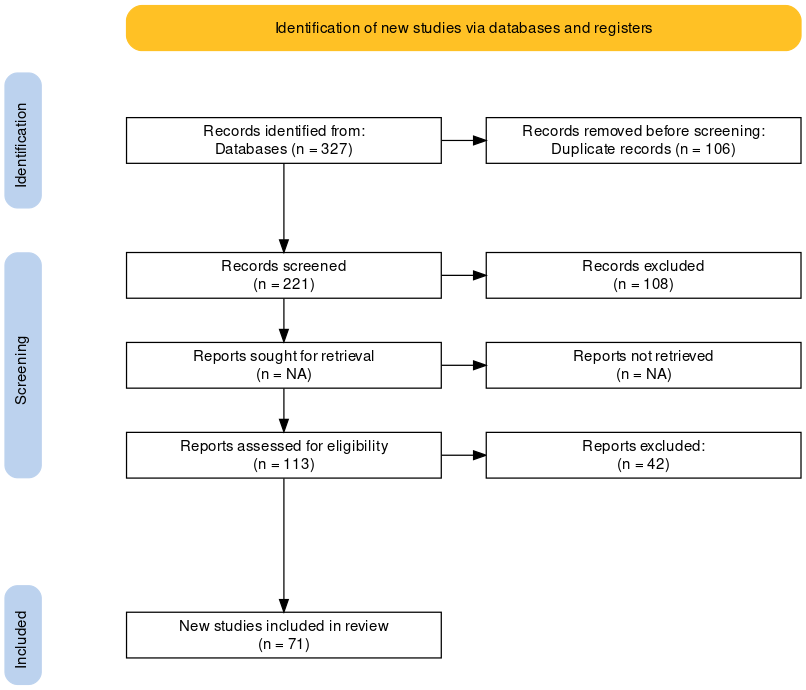
\includegraphics[width=0.9\linewidth]{figures/prisma_fc} \caption{PRISMA flow chart of this systematic literature review.}\label{fig:prisma-flowchart}
\end{figure}

\hypertarget{data-extraction-and-analysis}{%
\section{Data Extraction and Analysis}\label{data-extraction-and-analysis}}

We focus the data extraction on the MRP-related plot. We manually create a metadata for each plot (included in the supplementary material). We will use this metadata to analyse the current reporting practices with MRP. This metadata will also ensure the reproducibility of the analysis and to maintain the transparency of the systematic literature review process.

We code the plots according to their type, i.e., communication (coded to 0) and diagnostic plot (coded to 1). For diagnostic plots, we examine whether the plots compare MRP with other estimates, which are:

\begin{enumerate}
\def\labelenumi{\arabic{enumi}.}
\tightlist
\item
  Raw (direct estimates or direct disaggregation);
\item
  Ground truth;
\item
  Weighted estimates;
\item
  Estimates from other MRP models, for example, a paper build several MRP models from various simulation scenarios or using different covariates;
\item
  Estimates from another study/survey;
\item
  Estimates from another method, for example comparing MRP with Bayesian Additive Tress with Post-Stratification(BARP).
\end{enumerate}

Plots that show a comparison of MRP with the above list would be coded to 1, otherwise coded to 0.
Diagnostic plots also categorised based on how they compare the performance of MRP. The five observed criteria are:

\begin{enumerate}
\def\labelenumi{\arabic{enumi}.}
\tightlist
\item
  Bias;
\item
  Mean Absolute Error (MAE);
\item
  Mean Square Error (MSE)/ Relative Mean Square Error (RMSE);
\item
  Standard Error (SE);
\item
  Correlation.
\end{enumerate}

Each plot is assessed based on the use of the performance metric. For each metric is scored based on whether it is used (coded 1) or not (coded 0).

We also review other features of the plot using the grammar in \texttt{ggplot2} \autocite{ggplot2} as a framework. The common grammar used in practice allows us to understand to what extend MRP models are effectively visualised. It is worth noting that there is no specific convention or well-documented recommendation on how data should be visualised as building a graph more often involves choice or preference \autocite{MIDWAY2020100141}. For example, there is no specific convention on which variable should be put on the x and y-axis in a scatter plot, even though it has been common knowledge to put the response variable on the y-axis and the explanatory variable on the x-axis. Hence, grammar assists us in evaluating well-formed graphics \autocite{layered-grammar}. In addition, \textcite{vanderplas} mention that classifying and comparing graphs according to their grammar is more robust and more elegant.

Accordingly, we examine the facet, geom, axis, color, and shape. For reproducibility, the metadata also contains the article's author/s, publication year, title, and corresponding figure number as it appeared in the article. After the extraction, we analyze the data using graphical visualization with \texttt{ggplot2} \autocite{ggplot2}. The result will be discussed in the following subsection.

\hypertarget{common-practices-in-mrp-visualisations}{%
\section{Common practices in MRP visualisations}\label{common-practices-in-mrp-visualisations}}

In this study, graphics are classified into two types, i.e., communication and diagnostic plots. A plot is classified as a communication plot if the plot's goal is solely to convey the MRP result. A diagnostic plot is used to understand the MRP estimate, and typically displays the MRP estimation by showing the performance metrics or compares it with other estimation methods. From 71 articles, we extract the data of 243 plots. 47.33 \% of these plots are diagnostics plots, while the remaining are communication plots.

\hypertarget{performance-metrics-used-in-mrp}{%
\subsection{Performance metrics used in MRP}\label{performance-metrics-used-in-mrp}}

According to \textcite{BotchkarevAlexei2019ANTD}, performance metrics is \emph{``a logical and mathematical construct designed to measure how close are the actual results from what has been expected or predicted''} RMSE and MAE are among the most common methods used in many studies \autocite{BotchkarevAlexei2019ANTD}. However, \textcite{WillmottCJ2005Aotm} states that RMSE should not be reported in any studies since it could be multi-interpreted because it does not describe average error alone and MAE is more appropriate metric. This argument is denied by \textcite{ChaiT2014Rmse} who argue that RMSE is not ambiguous and better than MAE if the distribution of model's error is normal. Accordingly, there is no single metric that fits all methods \autocite{ChaiT2014Rmse}.

\begin{figure}
\centering
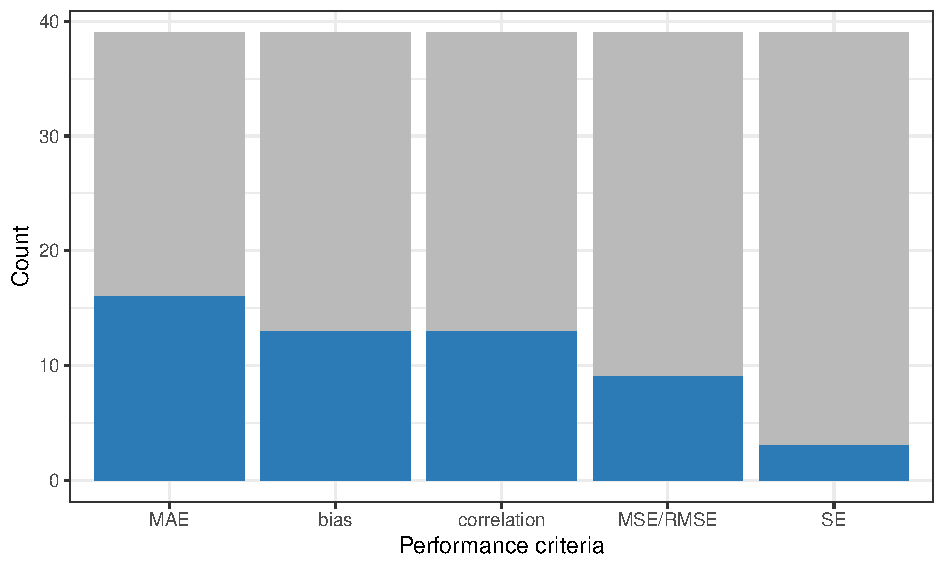
\includegraphics{thesis_files/figure-latex/perform-plot-1.pdf}
\caption{\label{fig:perform-plot}We observed five performance metrics used: Mean Absolute Error (MAE), bias, correlation, Mean Square Error/Root Mean Square Error (MSE/RMSE), and Standard Error (SE). The blue shade represents the number of articles that show performace metrics in plot, while the grey shade represents the number of articles that show performance of MRP but did not use the corresponding metrics.}
\end{figure}

In this study, we find that there are 39 plots out of 115 diagnostic plots (about 34\%) that display performance measures. As seen in Figure \ref{fig:perform-plot}, we find that MAE is the most widely used performance metric in MRP visualisations. Bias, which is interpreted similarly to MAE, is also widely used. Meanwhile, the squared error measures, which are MSE/RMSE and standard error, are only used in a few plots. It is interesting that correlation, which is not a common metric for performance, is more widely used than square error metrics.

Most of these metrics only refer to point estimates, i.e., the distance between the predicted value and the actual values. Also, these metrics mainly measure bias. However, MRP is a model in which bias-variance is applied. Therefore, other measures are also needed that reflect the degree of uncertainty and variations in the predicted value. Measures such as length of confidence or credibility interval can be used, in which the narrower the value, the more precise the estimates.

\hypertarget{common-comparisions-with-mrp}{%
\subsection{Common comparisions with MRP}\label{common-comparisions-with-mrp}}

The goal of MRP is to make a population estimate. The method aims to adjust an unrepresentative survey to obtain accurate population and sub-population estimates. Where possible MRP is usually compared with a true value. This is generally only possible in political science applications where an election provides this true estimate. To understand how MRP improves estimates from an unrepresentative survey when compared with no adjustment, MRP estimates are usually compared with direct estimates (raw). Similarly, to understand the improvement of estimates when compared with more traditional methods, MRP is often compared with weighted estimates.

\begin{figure}
\centering
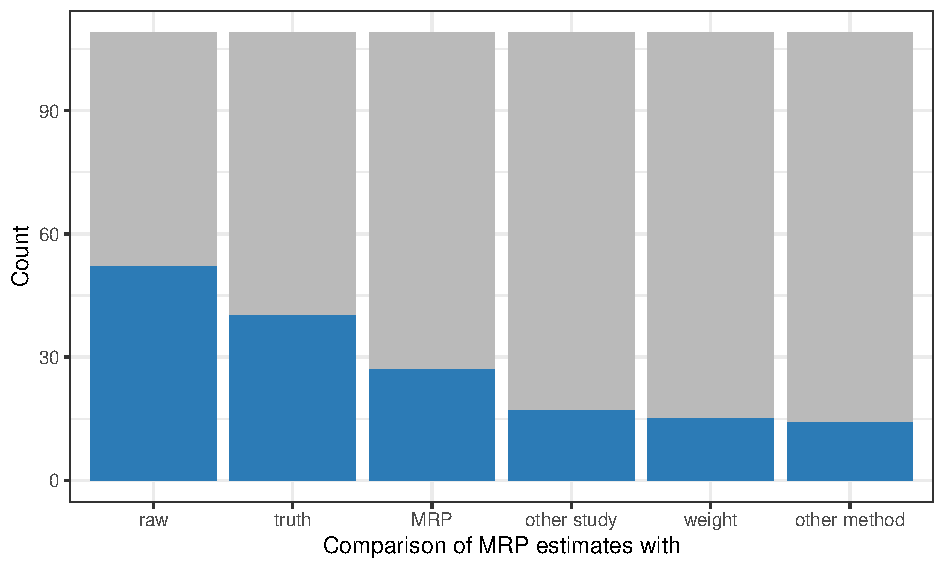
\includegraphics{thesis_files/figure-latex/compare-plot-1.pdf}
\caption{\label{fig:compare-plot}Estimates that are compared with MRP. The blue shade represents the number of articles that compare MRP estimates with the result of other estimation methods, while the grey shade represents the number of articles that also showed comparison of MRP but did not compare to this particular estimate. Note that the blue bars do not sum to the count because some plots compared to multiple alternative estimates.}
\end{figure}

This study finds that from 115 diagnostic plots, 109 (about 95\%) compare MRP estimates with estimates from other methods. Figure \ref{fig:compare-plot} shows the distribution of alternative estimates. MRP estimates are mostly compared to direct estimates and the ground truth. Some studies also compare estimates from several MRP models (usually with different model specifications). There are not many plots showing the comparison between MRP estimates and weighted estimates.

\hypertarget{common-grammar-in-mrp-visualisations}{%
\subsection{Common grammar in MRP visualisations}\label{common-grammar-in-mrp-visualisations}}

\textbf{Plot type}

\begin{figure}
\centering
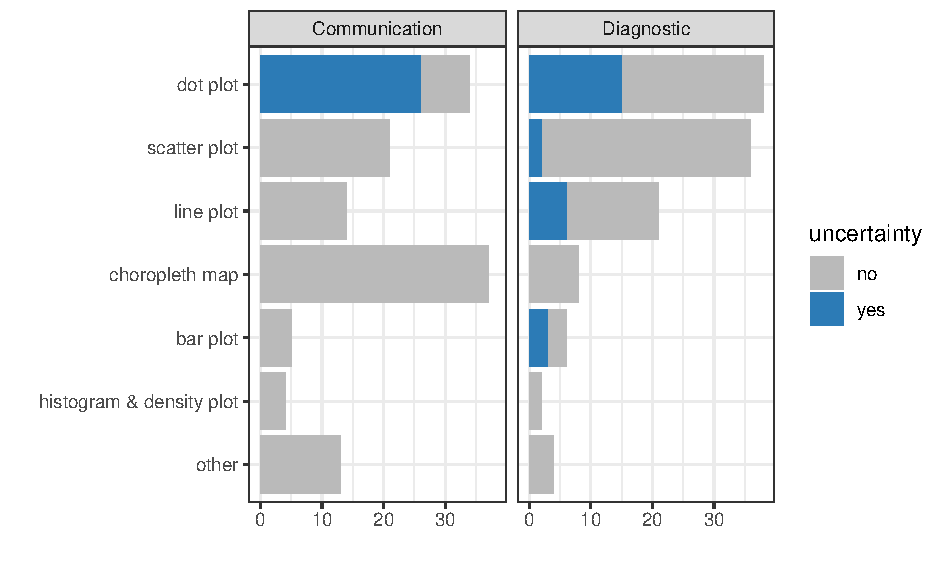
\includegraphics{thesis_files/figure-latex/common-plots-1.pdf}
\caption{\label{fig:common-plots}Common plot types used in MRP visualisations. The blue shade display the number of plots that showed uncertainty, while the grey shade display the number of plots that did not show uncertainty. Both communication and diagnostics plots rarely displayed uncertainty.}
\end{figure}

Plot type, referred to as \texttt{geom} in the grammar of graphics, represents the shape and features displayed in the graph. Figure \ref{fig:common-plots} suggests that communication and diagnostic plots have a different pattern in which plot types are used. Communicating MRP estimates are mostly done using a choropleth map as MRP is often used for small area estimation. For diagnostic purposes, dot plots are mostly used to compare more than two estimation methods or to show some performance metrics.

Notice that Figure \ref{fig:common-plots} also displays the use of uncertainty in MRP model visualisations. According to \textcite{MIDWAY2020100141}, displaying uncertainty in the statistical graphs is essential as the absence of this measure would produce a misleading interpretation and hinder some statistical messages. However, he further states that uncertainty is often neglected in data visualisation. This is what we find in this study - uncertainty is not often seen in the plots. This is possibly because many of the application areas are more familiar with official statistics. In official statistics uncertainty is often unreported because results that are not sufficiently precise are not reported.

\textbf{Values put in x and y-axis}

The main component of a data visualisation is the axis. x and y-axis represents what value/data are exactly displayed in the graph. In MRP visualisations (Figure \ref{fig:common-axis}), estimates, small area, actual value (truth), and time are amoung the values that are displayed in the plot. We can also see that the constructs represented by the x and y-axis are more varied in diagnostic plots. It is worth noting that there are no strict rules on values to put in x and y-axis. However, it is a common that the the fixed value is represented by the x-axis, while the random variable is represented in the y-axis. We do not see this in our results as we find estimates and truth are plotted on the x and y axes interchangeably. Another common rule of thumb is that time is almost always represented on the x-axis, which is supported by the findings of our study.

\begin{figure}
\centering
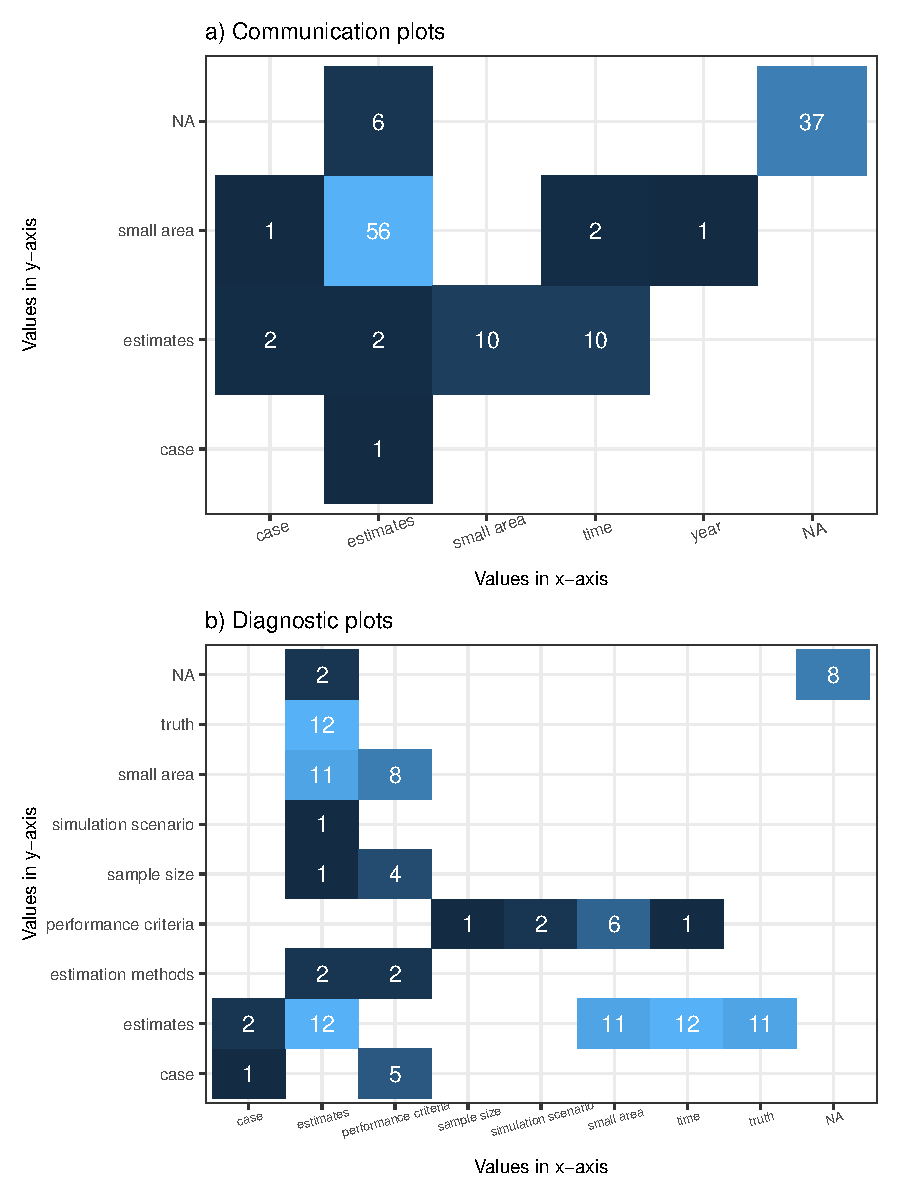
\includegraphics{thesis_files/figure-latex/common-axis-1.pdf}
\caption{\label{fig:common-axis}Common values put in plots' axis. Axis in diagnostic plots more varied compared to communication plot.}
\end{figure}

\textbf{Facet}

Paneling or faceting is considered as to one of the effective visualisation techniques to compare the same variables by its grouping factor \autocite{MIDWAY2020100141}. We find in our results that faceting is a common practice in MRP visualisations. Figure \ref{fig:facet-plots} shows that faceting the plots by small area that is being estimated is the most common, followed by case. Small area refers to the levels of the predictors in the MRP model, for example, state, county, and religion. In several plots, small area could be referred to another variable that is associated with the MRP estimates, but is not included in the model, such as the association between health literacy and the opinion on a health-related bill. Health literacy is a variable that is not included in fitting the MRP model, while the latter is the MRP estimates. Further, case is referred to the outcome predicted with MRP.

\begin{figure}
\centering
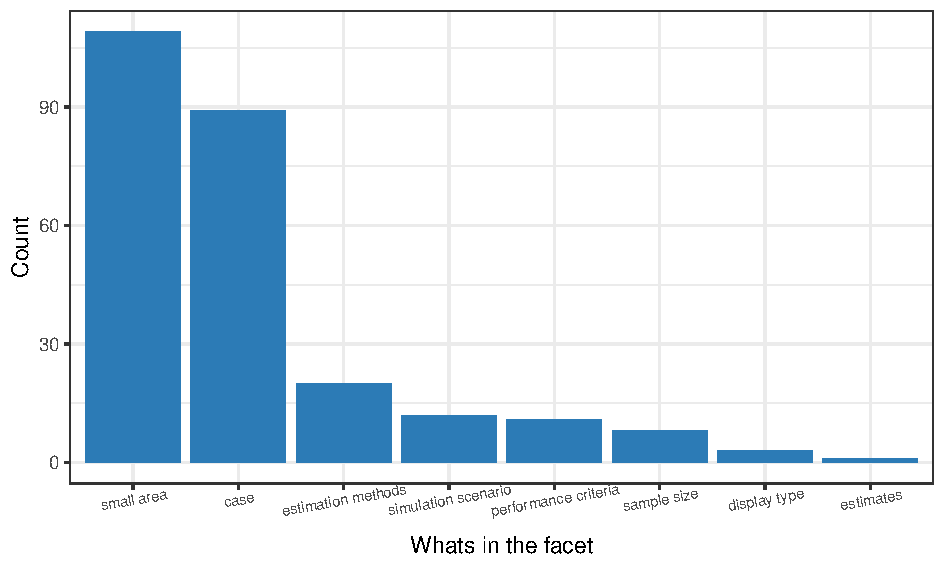
\includegraphics{thesis_files/figure-latex/facet-plots-1.pdf}
\caption{\label{fig:facet-plots}The facetting variable in MRP visualisations}
\end{figure}

\textbf{Other features used}

Besides the features explained previously, color and shape are also the components of grammar of graphics. According to a large experimental study on visualisations, color is a memorable feature of a graph \autocite{MIDWAY2020100141}. Further, \textcite{few_2008} states that the aim of color in data visualisations are to highlight particular data, to group items, and to encode quantitative values. In addition, color is sometimes displayed along with shapes to distinguish more features.

We find, as shown in Figure \ref{fig:sankey-feature}, that both communication and diagnostic plots incorporate color only about half the time. Shape is used less often. When there is only one feature to be displayed, for example, estimation methods, people tend to choose to use color first, rather than shape. This is seen in Figure \ref{fig:sankey-feature} as after incorporating color to distinct estimates, small area, estimation methods, and performance criteria, people tend to not use shape anymore.

\begin{figure}
\centering
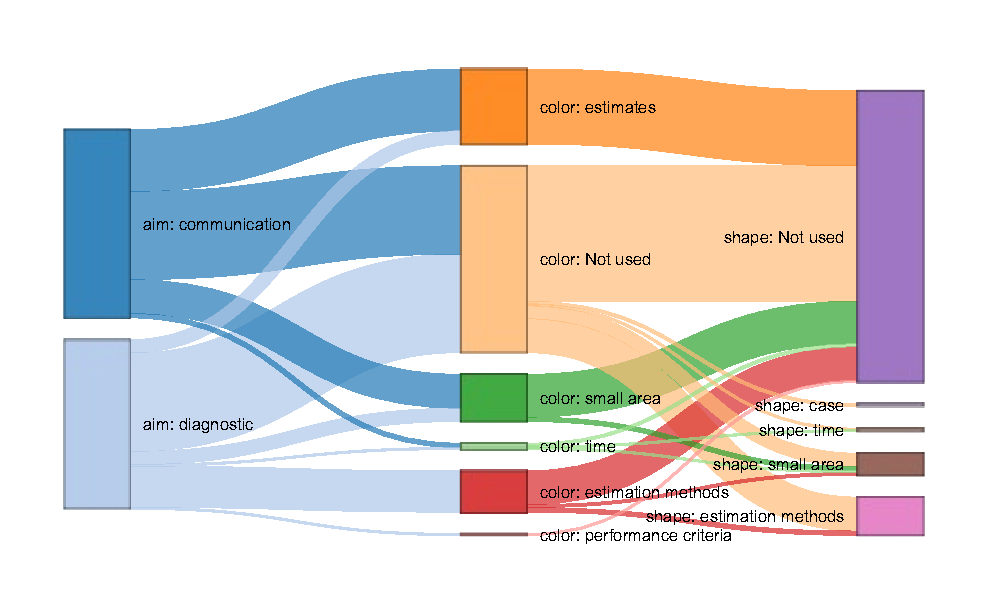
\includegraphics{thesis_files/figure-latex/sankey-feature-1.pdf}
\caption{\label{fig:sankey-feature}Color and shape commonly used in MRP visualisations. Both communication and diagnostic plots rarely use color and shape features.}
\end{figure}

\hypertarget{case-study-application-of-mrp-in-presidential-voting-estimation}{%
\chapter{Case Study: Application of MRP in Presidential Voting Estimation}\label{case-study-application-of-mrp-in-presidential-voting-estimation}}

The majority of MRP applications are used in the context of estimating public opinion in the social and political sciences, although, in recent development, MRP is also conducted in various fields, for example, health and environmental studies. When first introduced by \textcite{Gelman97poststratificationinto}, MRP was applied to generate state estimation of the 1988 U.S. presidential election. Additionally, various subsequent studies also made presidential voting the case of interest. We recorded at least seven articles (\textcite{GelmanAndrew2014HBAC}; \textcite{GhitzaYair2013DIwM}; \textcite{KiewietdeJongeChadP2018PSPE}; \textcite{LauderdaleBenjaminE2020Mppf}; \textcite{LeiRayleigh2017T2EA}; \textcite{ParkDavidK2004BMEw}; \textcite{WangWei2015Fewn}) included in the Systematic Literature Review in Chapter 2 have applied MRP in the case of the presidential election. Therefore, in this chapter, we will also apply MRP to estimate the 2016 U.S. presidential voting outcome, especially the probability of Trump votes. This also allows us to compare MRP estimates with the actual value of the Trump votes that are already available. In this case study, we use the Cooperative Congressional Election Study (CCES) 2016 data \autocite{cces_data} as the survey data and the American Community Survey data 2015-2017 \autocite{acs_data} as the population/ post-stratification data.

\hypertarget{data}{%
\section{Data}\label{data}}

\hypertarget{cooperative-congressional-election-study-cces-2016}{%
\subsection{Cooperative Congressional Election Study (CCES) 2016}\label{cooperative-congressional-election-study-cces-2016}}

CCES is an annual survey aims to capture Americans' view on Congress, their voting behavior and experience with regards to political geography, social, and demographic context \autocite{cces_data}. In 2016, CCES covers 64,600 samples spread over 51 states. Accordingly, \textcite{cces_data} mention that the data is precise enough to measure the distribution of voters' preference in most states. In addition, beyond its reliable sample size, CCES is deemed to be desirable dataset as it measures vote preference before and after in two waves so that it is even more reliable compared to generic question \autocite{kuriwaki}.

To fit MRP models, we use several variables from this survey. To obtain the data from the CCES website, we utilize an R package, \texttt{ccesMRPprep} \autocite{ccesmrpprep}. One of the advantages of using this package is that the data has been pre-processed in particular for MRP purposes, in this case, we use the \texttt{ccc\_std\_demographics} function. Also, the variable names are already recoded so it has a more interpretable names. The code to get the data is available in the supplementary materials of this thesis.

The outcome variables, which will be explained in detail in Section \ref{spec}, are the vote preference/intention (\texttt{CC16\_364c}), candidate voted (\texttt{CC16\_410a}), and party identity (\texttt{pid3} including leaners, i.e, coded as Independents in pid3 who expressed leaning towards a party in \texttt{pid7}). Table \ref{tab:outcome-table} shows the distribution of answers in those three variables. In \texttt{ccesMRPprep}, these variables have been renamed so that they are equivalent to \texttt{intent\_pres\_16}, \texttt{voted\_pres\_16}, and \texttt{pid3\_leaner}, respectively. It is worth noting that the MRP models we would like to build use binary responses. Hence, these variables are recoded into yes/no in terms of whether the respondents vote for Trump/Republican or not.

\begin{table}
\caption{\label{tab:outcome-table}Percentage of each answer in CCES 2016. This question will be the MRP models outcome in this case study. Since the model outcome is binary, these answer will be converted to be yes/no in the context of vote for Trump/Republican.}

\centering
\begin{tabular}[t]{lr}
\toprule
Candidate voted & percentage\\
\midrule
Hilary Clinton & 34.27\\
Donald Trump & 29.03\\
Other / Someone Else & 6.26\\
Did Not Vote & 0.13\\
Not Sure / Don't Recall & 0.35\\
\addlinespace
NA & 29.97\\
\bottomrule
\end{tabular}
\centering
\begin{tabular}[t]{lr}
\toprule
Candidate will be voted & percentage\\
\midrule
Donald Trump (Republican) & 29.76\\
Hillary Clinton (Democrat) & 42.57\\
Gary Johnson (Libertarian) & 4.87\\
Jill Stein (Green) & 2.17\\
Other & 2.91\\
\addlinespace
I Won't Vote in this Election & 5.13\\
I'm Not Sure & 10.12\\
NA & 2.47\\
\bottomrule
\end{tabular}
\centering
\begin{tabular}[t]{lr}
\toprule
Party identity including leaners & percentage\\
\midrule
Democrat (Including Leaners) & 48.20\\
Republican (Including Leaners) & 32.27\\
Independent (Excluding Leaners) & 16.24\\
Not Sure & 3.20\\
NA & 0.08\\
\bottomrule
\end{tabular}
\end{table}

Further, the geography and demographic variables used as covariates in the models are \texttt{state}, \texttt{age}, \texttt{gender}, \texttt{education}, and \texttt{race}. Table \ref{tab:covariate-tables} shows the distribution of categories/levels of \texttt{age}, \texttt{gender}, \texttt{education}, and \texttt{race}. Initially, age is a discrete variable but in this case it is categorised. Also, \texttt{education} and \texttt{race} has more levels in the original data but it is collapsed here to obtain fewer levels. The proportion of people answered the survey based on the state is displayed in the appendix of this thesis.

\begin{table}
\caption{\label{tab:covariate-tables}The response of covariates. Note that this response has been categorised into certain levels that are reflected in these tables.}

\centering
\begin{tabular}[t]{lr}
\toprule
Gender & percentage\\
\midrule
Male & 45.71\\
Female & 54.29\\
\bottomrule
\end{tabular}
\centering
\begin{tabular}[t]{lr}
\toprule
Race & percentage\\
\midrule
White & 69.44\\
Black & 12.00\\
Hispanic & 10.59\\
Asian & 3.53\\
Native American & 0.81\\
\addlinespace
All Other & 3.63\\
\bottomrule
\end{tabular}
\centering
\begin{tabular}[t]{lr}
\toprule
Age & percentage\\
\midrule
18 to 24 years & 8.30\\
25 to 34 years & 19.62\\
35 to 44 years & 15.75\\
45 to 64 years & 38.36\\
65 years and over & 17.98\\
\bottomrule
\end{tabular}
\centering
\begin{tabular}[t]{lr}
\toprule
Education & percentage\\
\midrule
HS or Less & 28.41\\
Some College & 35.38\\
4-Year & 23.04\\
Post-Grad & 13.17\\
\bottomrule
\end{tabular}
\end{table}

\hypertarget{american-community-survey-acs-2015-2017}{%
\subsection{American Community Survey (ACS) 2015-2017}\label{american-community-survey-acs-2015-2017}}

In this study, we use the ACS 2015-2017 data as the post-stratification data. The ACS provides annual-basis information about jobs and occupations, demographic and citizenship, educational attainment, homeownership, and other topics \autocite{acs_data_about}. Further, the ACS uses monthly probabilistic samples to produce the annual estimates. It could be understood that the ACS is desirable data to represent the U.S. population since the coverage rate for the 2015-2017 ACS is 92.4\%, 91.9\%, 91.6\%, respectively \autocite{acs_coverage_rate}. It is also implied by \textcite{GaoYuxiang2021IMRa} that the ACS is the most accurate representation of the U.S. population every year.

To fit MRP models, we need the individual data of the ACS instead of the aggregated statistics. Hence, we use the 1-year Public Use Microdata Sample (PUMS), which carries the information/records of individual people on a yearly basis. The 1-year PUMS data reflects approximately one percent of the U.S. population \autocite{pums_metadata}. Therefore, in this study, we use three years periods of the ACS 1-Year PUMS from 2015-2017 instead of 2016 only to get a better and more stable representation of the American population. Every individual in the data has a weight (\texttt{PWGTP}). Since we use three years period, this weight is then divided by 3.

The data is publicly available on the \href{https://www.census.gov/programs-surveys/acs/microdata/access.2015.html}{U.S. Census Bureau website}. We downloaded the data in a .csv format (csv\_pus.zip) year by year (2015-2019) through access on \href{https://www2.census.gov/programs-surveys/acs/data/pums/2015/1-Year/}{FTP site}. After that, we did a data pre-processing to bind the three years of the PUMS data. We only use some variables in this data for the MRP-purposes, i.e., unique identifier of the person (\texttt{SERIALNO}), state (\texttt{ST}), weight (\texttt{PWGTP}), education (\texttt{SCHL}), sex (\texttt{SEX}), race (\texttt{RAC1P}), Hispanic origin (\texttt{HISP}), and age (\texttt{AGEP}). We also did a data munging to recode and collapse some categories in these variables. Note that the \texttt{RAC1P} did not record for Hispanic ethnicity. Hence, we introduce a new category here, Hispanic, identified if the person answers other than ``1'' in the \texttt{HISP} variable. Table \ref{tab:acs-response-freq} shows the categorised response of the variables obtained from the ACS, i.e., age, race and ethnicity, and education. Also, notice that we get some NA values in education. This is actually the education level of under-school-age respondents. In fact, we will omit the ``Less than 18 years'' age group in the MRP models as it is not included in the survey data (CCES). Hence, the NAs in education response will be eventually omitted as well. The detailed code of the data pre-processing is available in the supplementary materials of this thesis.

\begin{table}
\caption{\label{tab:acs-response-freq}The response categories of post-stratification data.}

\centering
\begin{tabular}[t]{lr}
\toprule
Sex & percentage\\
\midrule
Male & 48.9\\
Female & 51.1\\
\bottomrule
\end{tabular}
\centering
\begin{tabular}[t]{lr}
\toprule
Race and ethnicity & percentage\\
\midrule
Black or African American alone & 9.89\\
Two or More Races & 2.24\\
White alone & 67.00\\
Asian alone & 5.16\\
Hispanic & 14.41\\
\addlinespace
American Indian alone & 0.80\\
Some Other Race alone & 0.19\\
Native Hawaiian and Other Pacific Islander alone & 0.15\\
American Indian and Alaska Native tribes & 0.08\\
Alaska Native alone & 0.07\\
\bottomrule
\end{tabular}
\centering
\begin{tabular}[t]{lr}
\toprule
Age & percentage\\
\midrule
Less than 18 years & 20.73\\
18-24 & 8.73\\
25-34 & 11.92\\
35-44 & 11.62\\
45-54 & 13.45\\
\addlinespace
55-64 & 14.64\\
65-74 & 10.95\\
75-89 & 7.00\\
90 years and over & 0.95\\
\bottomrule
\end{tabular}
\centering
\begin{tabular}[t]{lr}
\toprule
Education & percentage\\
\midrule
No high school & 27.03\\
Regular high school diploma & 18.82\\
Some college & 21.25\\
Associate's degree & 6.39\\
Bachelor's degree & 14.50\\
\addlinespace
Post-graduate & 8.99\\
NA & 3.03\\
\bottomrule
\end{tabular}
\end{table}

\hypertarget{spec}{%
\section{Model Specifications}\label{spec}}

In Chapter 2, we found that the diagnostic plots shown in many articles compare MRP estimates with other estimates, one of which compares several MRP estimates with different specifications. Therefore, in this case study, we build five different MRP models as follows.

\newpage

\textbf{Baseline model}

We begin the model fitting with the baseline model. In this model, we set the binary outcome as whether the respondents vote for Trump or not in the 2016 election. Therefore, we transform the response of \texttt{voted\_pres\_16} into a binary variable called \texttt{vote}. The covariates used are \texttt{age}, \texttt{gender}, \texttt{state}, and the re-categorised/collapsed \texttt{race} variable into fewer levels. As seen in Table \ref{tab:covariate-tables}, \texttt{race} has 6 categories, i.e., \texttt{White}, \texttt{Black}, \texttt{Hispanic}, \texttt{Asian}, \texttt{Native\ American}, and \texttt{All\ Other}. In the baseline model, we collapsed the \texttt{Native\ American} and \texttt{All\ Other} into \texttt{Other}. Hence, the baseline model equation is:

\begin{equation} 
\begin{split}
\Pr(vote_{j[i]} = 1) = logit^{-1}\left(\beta_0 + \alpha^{age}_{j[i]} + \alpha^{gender}_{j[i]} + \alpha^{state}_{j[i]} + \alpha^{collapsed\ race}_{j[i]}\right), for\ i = 1, ...., n, 
\end{split}
\label{eq:baseline-model}
\end{equation}

and \(vote_{j[i]}\) is the observed binary outcome (1 = yes, 0 = no) for individual \(i\) in post-stratification cell \(j\). \(\beta_0\) is the intercept. \(\alpha^{age}_{j[i]}\), \(\alpha^{gender}_{j[i]}\), \(\alpha^{state}_{j[i]}\), and \(\alpha^{collapsed\ race}_{j[i]}\) are the random effects for \texttt{age}, \texttt{gender}, \texttt{state}, and \texttt{collapsed\ race}, respectively. The subscript in each coefficient represents the category of the \(i-th\) respondent, such as, \(\alpha^{collapsed\ race}_{j[i]}\) takes value from \{\(\alpha^{collapsed\ race}_{White}\), \(\alpha^{collapsed\ race}_{Black}\), \(\alpha^{collapsed\ race}_{Hispanic}\), \(\alpha^{collapsed\ race}_{Asian}\), and \(\alpha^{collapsed\ race}_{Other}\)\}. Each random effect has an independent prior distribution, such as, \(\alpha^{collapsed\ race}_{j}\) \textasciitilde{} \(N(0, \sigma^2_{collapsed\ race})\).

\vspace{\baselineskip}

\textbf{Model with \texttt{education} as additional covariate}

Next, we create a bigger model by adding \texttt{education} as additional covariate to the baseline model. Hence, the model specification is:

\begin{equation} 
\begin{split}
\Pr(vote_{j[i]} = 1) &= logit^{-1}\left(\beta_0 + \alpha^{age}_{j[i]} + \alpha^{gender}_{j[i]} + \alpha^{state}_{j[i]} + \alpha^{collapsed\ race}_{j[i]} + \alpha^{education}_{j[i]}\right), \\
for\ i &= 1, ...., n.
\end{split}
\label{eq:model2}
\end{equation}

\vspace{\baselineskip}

\textbf{Model with original race categories}

This model is essentially the same with baseline model, except that there are more race categories, which are \texttt{White}, \texttt{Black}, \texttt{Hispanic}, \texttt{Asian}, \texttt{Native\ American}, and \texttt{All\ Other}. The model equation is:

\begin{equation} 
\begin{split}
\Pr(vote_{j[i]} = 1) = logit^{-1}\left(\beta_0 + \alpha^{age}_{j[i]} + \alpha^{gender}_{j[i]} + \alpha^{state}_{j[i]} + \alpha^{original\ race}_{j[i]}\right), for\ i = 1, ...., n.
\end{split}
\label{eq:model3}
\end{equation}

\textbf{Model with different outcomes}

\textbf{Vote intention/preference}

This model mimicks the model in Equation \eqref{eq:model2}, except that we have different outcome or response variable. The response here is whether the respondent intent to vote for Trump (\texttt{yes}) or not (\texttt{no}). It is transformed from \texttt{intent\_pres\_16} variable in the CCES data. The model is specified as follows:

\begin{equation} 
\begin{split}
\Pr(intent_{j[i]} = 1) &= logit^{-1}\left(\beta_0 + \alpha^{age}_{j[i]} + \alpha^{gender}_{j[i]} + \alpha^{state}_{j[i]} + \alpha^{collapsed\ race}_{j[i]} + \alpha^{education}_{j[i]}\right), \\
for\ i &= 1, ...., n.
\end{split}
\label{eq:model4a}
\end{equation}

\textbf{Party identity}

Beside vote intention, another outcome is the party identity in terms of whether the respondents identify themselves as Republican or not. This variable is derived from \texttt{pid3\_leaner} variable. The specification of covariates is also the same with model in Equation \eqref{eq:model2}.

\begin{equation} 
\begin{split}
\Pr(party_{j[i]} = 1) &= logit^{-1}\left(\beta_0 + \alpha^{age}_{j[i]} + \alpha^{gender}_{j[i]} + \alpha^{state}_{j[i]} + \alpha^{collapsed\ race}_{j[i]} + \alpha^{education}_{j[i]}\right), \\
for\ i &= 1, ...., n.
\end{split}
\label{eq:model4b}
\end{equation}

\hypertarget{prep}{%
\section{Model Preparation and Fitting}\label{prep}}

The MRP models require a synchronous survey and population data. Hence, to achieve this, we need to map the survey data to the population data. In this study, the model preparation and survey-population data mapping conducted with an R package, \texttt{mrpkit} \autocite{mrpkit}. This package allows the transparent and reproducible workflow to build MRP model, from the data mapping until the prediction stage, including the model specification setting. The detailed code to build the MRP models is available in the supplementary materials of this thesis.

After mapping the survey and population data, we can obtain the post-stratification table displayed in Table \ref{tab:post-strat-table}

\begin{table}

\caption{\label{tab:post-strat-table}First five rows of the post-stratification table}
\centering
\begin{tabular}[t]{llllllr}
\toprule
age & state & gender & collapsed\_re & original\_re & education & N\_j\\
\midrule
18 to 24 years & Alabama & Male & Black & Black & HS or Less & 40443.3333\\
18 to 24 years & Alabama & Male & Black & Black & Some College & 31610.3333\\
18 to 24 years & Alabama & Male & Black & Black & 4-Year & 1760.3333\\
18 to 24 years & Alabama & Male & Black & Black & Post-Grad & 158.3333\\
18 to 24 years & Alabama & Male & Other & All Other & HS or Less & 2464.3333\\
\bottomrule
\end{tabular}
\end{table}

Next, we implement Bayesian multilevel model using \texttt{brms} \autocite{brms} to fit the model and obtain the posterior distributions of the parameters. \texttt{brms} itself incorporates cmdstanr \autocite{cmdstanr} as the backend. The samples of posterior distribution are generated in 4 chains with 1000 iterations in each chain. Since this task is computationally heavy and time-consuming, we conduct it using \href{https://docs.monarch.erc.monash.edu/MonARCH/aboutMonArch.html}{Monash's High Performance Cluster (HPC) infrastructure}.

\hypertarget{results-and-discussion}{%
\section{Results and Discussion}\label{results-and-discussion}}

\appendix

\hypertarget{appendix}{%
\chapter{Appendix}\label{appendix}}

You might put some computer output here, or maybe additional tables.

Note that line 5 must appear before your first appendix. But other appendices can just start like any other chapter.

\printbibliography[heading=bibintoc]



\end{document}
